%%%%%%%%%%%%%%%%%%%%%%%%%%%%%%%%%%%%%%%%%%%%%%%%%%%%%%%%%%%%%%%%%%%%%%%%%%%%%%%%
% TUM-Vorlage: Präsentation
%%%%%%%%%%%%%%%%%%%%%%%%%%%%%%%%%%%%%%%%%%%%%%%%%%%%%%%%%%%%%%%%%%%%%%%%%%%%%%%%
%
% Rechteinhaber:
%     Technische Universität München
%     https://www.tum.de
% 
% Gestaltung:
%     ediundsepp Gestaltungsgesellschaft, München
%     http://www.ediundsepp.de
% 
% Technische Umsetzung:
%     eWorks GmbH, Frankfurt am Main
%     http://www.eworks.de
%
%%%%%%%%%%%%%%%%%%%%%%%%%%%%%%%%%%%%%%%%%%%%%%%%%%%%%%%%%%%%%%%%%%%%%%%%%%%%%%%%


%%%%%%%%%%%%%%%%%%%%%%%%%%%%%%%%%%%%%%%%%%%%%%%%%%%%%%%%%%%%%%%%%%%%%%%%%%%%%%%%
% Zur Wahl des Seitenverhältnisses bitte einen der beiden folgenden Befehle
% auskommentieren und den ausführen lassen:
% \input{./Ressourcen/Praesentation/Praeambel4zu3.tex} % Seitenverhältnis 4:3
\input{./Ressourcen/Praesentation/Praeambel16zu9.tex} % Seitenverhältnis 16:9
%%%%%%%%%%%%%%%%%%%%%%%%%%%%%%%%%%%%%%%%%%%%%%%%%%%%%%%%%%%%%%%%%%%%%%%%%%%%%%%%


%%%%%%%%%%%%%%%%%%%%%%%%%%%%%%%%%%%%%%%%%%%%%%%%%%%%%%%%%%%%%%%%%%%%%%%%%%%%%%%%
\input{./_Einstellungen.tex}                    % !!! DATEI ANPASSEN !!!
%%%%%%%%%%%%%%%%%%%%%%%%%%%%%%%%%%%%%%%%%%%%%%%%%%%%%%%%%%%%%%%%%%%%%%%%%%%%%%%%


\tikzset{
    key/.pic={
      \filldraw (2.7,1) coordinate (-name) -- ++(-7, 0) -- ++(-1,-1) -- ++(1, -1) -- ++(0.5, 0.5) -- ++(0.5, -0.5) -- ++(0.75, 0.75) -- ++(0.75, -0.75) -- ++(0.5, 0.5) -- ++(0.5, -0.5) -- ++(1, 1) -- ++(1, -1) -- ++(0.5, 0.5) -- ++(0.5, -0.5) -- ++(0.5, 0) arc (-180+30:180-30:2) -- cycle;
    }
  }
  
  \tikzset{
    lock/.pic={    
      \fill[even odd rule] (-2.5, 0) -- ++(0,3) -- ++(0.5,0) -- ++(0,1) arc (180:0:2) -- ++(0,-1) -- ++(0.5,0) -- ++(0,-3) -- ++(-5, 0) ++(1, 3) -- ++(0,1) arc (180:0:1.5) -- ++(0,-1) -- ++(-3,0);
    }
  }  
  
  \tikzset{
    tree/.pic={    
      \scoped[sibling distance=20, level distance=12, inner sep=1]{
        \tikzstyle{every node}=[fill, circle, draw, anchor=center];
        \tikzstyle{level 2}=[sibling distance=6];
        \fill (0,0.5) node (root) [anchor=south] {} child {node (b) {} child {node {}} child {node {}} child {node {}}} child { node {} child {node {}}};
      };  
    }
  }   
  

\renewcommand{\PersonTitel}{}
\newcommand{\Datum}{\today}

\renewcommand{\PraesentationFusszeileZusatz}{| Bachelor's Thesis | Implementation of ABE in Rust on ARM Cortex M Processors}

\title{Implementation of Attribute-Based Encryption in Rust on ARM Cortex M Processors}
\author{\PersonTitel{} \PersonVorname{} \PersonNachname}
\institute[]{\UniversitaetName \\ \FakultaetName \\ \LehrstuhlName}
\date[\Datum]{Munich, April 7th, 2021}
\subject{Implementation of Attribute-Based Encryption in Rust on ARM Cortex M Processors}


%%%%%%%%%%%%%%%%%%%%%%%%%%%%%%%%%%%%%%%%%%%%%%%%%%%%%%%%%%%%%%%%%%%%%%%%%%%%%%%%
\input{./Ressourcen/Praesentation/Anfang.tex} % !!! NICHT ENTFERNEN !!!
%%%%%%%%%%%%%%%%%%%%%%%%%%%%%%%%%%%%%%%%%%%%%%%%%%%%%%%%%%%%%%%%%%%%%%%%%%%%%%%%


%%%%%%%%%%%%%%%%%%%%%%%%%%%%%%%%%%%%%%%%%%%%%%%%%%%%%%%%%%%%%%%%%%%%%%%%%%%%%%%%
% FOLIENSTIL: Standard
\PraesentationMasterStandard

\PraesentationTitelseite % Fügt die Startseite ein

\begin{frame}
    \frametitle{Table of Contents}
    \tableofcontents[hideallsubsections]
\end{frame}

\section{Introduction}

\begin{frame}[c]
    \frametitle{What did I do?}

    \begin{center}
        \begin{tikzpicture}[brace/.style={decorate, decoration={brace, amplitude=10pt}}, lbl/.style={midway, anchor=south, align=center}]
            \node[align=center, font=\LARGE] (name) at (0, 0) {\textcolor{TUMBlauDunkel}{Implementation} of \textcolor{TUMOrange}{Attribute-Based} \textcolor{TUMGruen}{Encryption} in Rust\\\textcolor{TUMBlauDunkel}{on ARM Cortex M Processors}};
            \draw[brace, color=TUMBlauDunkel] (-8.25,1) -- (-3,1) node [lbl, yshift=0.5cm] {Implementation of embedded\\ABE library + Evaluation:\\Does this even make\\sense on a small MCU?};
            \draw[brace, color=TUMOrange] (-2.6,1) -- (2.5, 1) node [lbl, yshift=0.5cm] {e.g. for a student:\\``is freshman''\\``has passed itsec''};
            \draw[brace, color=TUMGruen] (2.75,1) -- (6, 1) node [lbl, yshift=0.5cm] {alternatives: standard\\symmetric and\\asymmetric crypto?!};
            \draw[brace] (6.5, 1) -- (8.75, 1) node [lbl, yshift=0.5cm, xshift=0.5cm] {memory-safety\\guarantees\\built-in!};
            \draw[brace, decoration={mirror}, color=TUMBlauDunkel] (-4.75, -1) -- (4.75, -1) node [lbl, yshift=-0.5cm, anchor=north] {Constrained MCUs!\\our SoC: 64MHz Cortex M4 with 256KB RAM};
        \end{tikzpicture}
    \end{center}
\end{frame}

\begin{frame}[c]
    \frametitle{What for?}
    \input{../thesis/figures/01_system_architecture}
\end{frame}

\begin{frame}[c]
    \frametitle{ABE vs. standard encryption}
    % 
\begin{figure} \centering
    \begin{subfigure}{.8\textwidth}
        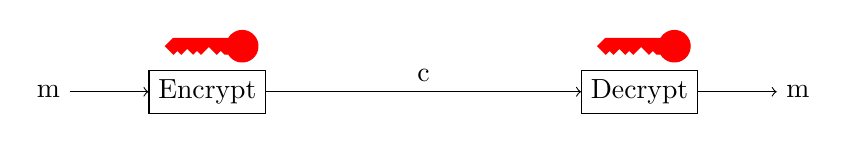
\begin{tikzpicture}
            \draw[->] (0, 0) node [anchor=east] {m} -- ++(1, 0) node (encrypt) [anchor=west, draw] {Encrypt};
            \path (encrypt.north) -- +(0, 0.3) pic [anchor=west, scale=0.1, red, fill=red] {key};
            \draw[->] (encrypt.east) -- ++(2, 0) node [anchor=south] {c} -- ++(2,0) node (decrypt) [anchor=west, draw] {Decrypt};
            \path (decrypt.north) -- +(0, 0.3) pic [anchor=west, scale=0.1, red, fill=red] {key};
            \draw[->] (decrypt.east) -- ++(1,0) node [anchor=west] {m};
        \end{tikzpicture}
        \caption{Symmetric Encryption: The same key is used for encryption and decryption. This key needs to be kept secret.} \label{fig:keys-symmetric}
    \end{subfigure}
    \\
    \vspace{0.5cm}
    \begin{subfigure}{.8\textwidth}
        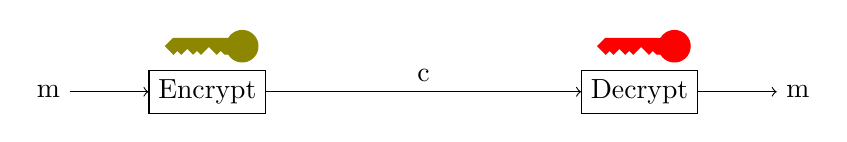
\begin{tikzpicture}
            \draw[->] (0, 0) node [anchor=east] {m} -- ++(1, 0) node (encrypt) [anchor=west, draw] {Encrypt};
            \path (encrypt.north) -- +(0, 0.3) pic [anchor=west, scale=0.1, olive, fill=olive] {key};
            \draw[->] (encrypt.east) -- ++(2, 0) node [anchor=south] {c} -- ++(2,0) node (decrypt) [anchor=west, draw] {Decrypt};
            \path (decrypt.north) -- +(0, 0.3) pic [anchor=west, scale=0.1, red, fill=red] {key};
            \draw[->] (decrypt.east) -- ++(1,0) node [anchor=west] {m};
        \end{tikzpicture}
        \caption{Asymmetric Encryption: Different keys for encryption and decryption. Decryption succeeds if and only if the decryption key is exactly the counterpart to the encryption key. Only the decryption key needs to be kept secret.} \label{fig:keys-asymmetric}
    \end{subfigure}
    \\ 
    \vspace{0.5cm}
    \begin{subfigure}{.8\textwidth}
        \begin{tikzpicture}[sibling distance=4mm, level distance=3mm]
            \draw[->] (0, 0) node [anchor=east] {m} -- ++(1, 0) node (encrypt) [anchor=west, draw] {Encrypt};
            
            \scoped{
                \tikzstyle{every node}=[fill, circle, draw, inner sep=0.5mm];
                \tikzstyle{level 2}=[sibling distance=1.5mm];
                \fill[red] (decrypt.north) -- ++(0, 0.7) node [anchor=south] {} child {node {} child {node {}} child {node {}} child {node {}}} child { node {} child {node {}}};
            };
            \draw[->] (encrypt.east) -- ++(2, 0) node [anchor=south] {c} -- ++(2,0) node (decrypt) [anchor=west, draw] {Decrypt};
            \path (encrypt.north) -- +(0, 0.3) node [olive] {$\{A, B, C\}$};
            \draw[->] (decrypt.east) -- ++(1,0) node [anchor=west] {m};
        \end{tikzpicture}
        \caption{\glslink{gls-kp-abe}{Key-Policy Attribute-Based Encryption}: Attributes for encryption, access structure for decryption. Decryption succeeds if and only if the attributes of the ciphertext satisfy the policy embedded in the key.} \label{fig:keys-abe}
    \end{subfigure}
    \\ 
    \vspace{0.5cm}
    \begin{subfigure}{.8\textwidth}
        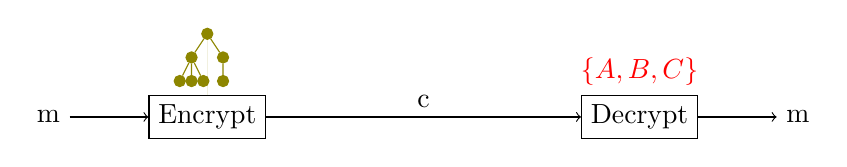
\begin{tikzpicture}[sibling distance=4mm, level distance=3mm]
            \draw[->] (0, 0) node [anchor=east] {m} -- ++(1, 0) node (encrypt) [anchor=west, draw] {Encrypt};
            
            \scoped{
                \tikzstyle{every node}=[fill, circle, draw, inner sep=0.5mm];
                \tikzstyle{level 2}=[sibling distance=1.5mm];
                \fill[olive] (encrypt.north) -- ++(0, 0.7) node [anchor=south] {} child {node {} child {node {}} child {node {}} child {node {}}} child { node {} child {node {}}};
            };
            \draw[->] (encrypt.east) -- ++(2, 0) node [anchor=south] {c} -- ++(2,0) node (decrypt) [anchor=west, draw] {Decrypt};
            \path (decrypt.north) -- +(0, 0.3) node [red] {$\{A, B, C\}$};
            \draw[->] (decrypt.east) -- ++(1,0) node [anchor=west] {m};
        \end{tikzpicture}
        \caption{\glslink{gls-cp-abe}{Ciphertext-Policy Attribute-Based Encryption}: \Gls{access-policy} for encryption, attributes for decryption. Decryption succeeds if and only if the attributes of the key match the policy embedded in the ciphertext.} \label{fig:keys-abe}
    \end{subfigure}
    \caption[Keys in different classes of encryption schemes]{Keys used for encryption and decryption in different classes of encryption schemes. Red information has to be kept secret, green information may be made publicly available. For the differences between the two types of \acrshort{abe}, see section~\ref{sec:cp-vs-kp}.}
    \label{fig:key-use}
\end{figure}
\end{frame}

%%%%%%%%%%%%%%%%%%%%%%%%%%%%%%%%%%%%%%%%%%%%%%%%%%%%%%%%%%%%%%%%%%%%%%%%%%%%%%%%
% FOLIENSTIL: Standard mit Lehrstuhl-, Fakultäts- und Universitätsnamen im
% Kopfbereich links
\section{Background}
\subsection{Attribute-Based Encryption}
% \PraesentationMasterKopfzeileDreizeiler

\subsection{Secret Sharing}

\subsection{Elliptic Curves}
% \PraesentationTitelseite

\section{Related Research}

\section{Implemented ABE Schemes}

\section{Implementation}

\section{Results}

%%%%%%%%%%%%%%%%%%%%%%%%%%%%%%%%%%%%%%%%%%%%%%%%%%%%%%%%%%%%%%%%%%%%%%%%%%%%%%%%
% FOLIENSTIL: Weisse Schrift auf blauem Grund
% \PraesentationMasterWeissBlau

%%%%%%%%%%%%%%%%%%%%%%%%%%%%%%%%%%%%%%%%%%%%%%%%%%%%%
%% Startseiten                                     %%

% Setzt die Startseite auf eine mit Flaggen als Hintergrund:
\PraesentationStartseiteFlaggen

% Setzt die Startseite auf eine mit mit einer Zeichnung des TUM-Uhrenturms:
%\PraesentationStartseiteUhrenturm

% Setzt die Startseite auf eine ohne Hintergrund:
%\PraesentationStartseiteLeer

\PraesentationTitelseite % Fügt die Startseite ein
%%%%%%%%%%%%%%%%%%%%%%%%%%%%%%%%%%%%%%%%%%%%%%%%%%%%%


\begin{frame}
    \PraesentationUeberschriftZweizeilig{Präsentationsmuster}{%
        kann auch als Kapiteltrenner verwendet werden}
\end{frame}

%%%%%%%%%%%%%%%%%%%%%%%%%%%%%%%%%%%%%%%%%%%%%%%%%%%%%%%%%%%%%%%%%%%%%%%%%%%%%%%%
% FOLIENSTIL: Weisse Schrift auf schwarzem Grund
\PraesentationMasterWeissSchwarz

\begin{frame}
    \frametitle{Präsentationsmuster}
\end{frame}


%%%%%%%%%%%%%%%%%%%%%%%%%%%%%%%%%%%%%%%%%%%%%%%%%%%%%%%%%%%%%%%%%%%%%%%%%%%%%%%%
\end{document} % !!! NICHT ENTFERNEN !!!
%%%%%%%%%%%%%%%%%%%%%%%%%%%%%%%%%%%%%%%%%%%%%%%%%%%%%%%%%%%%%%%%%%%%%%%%%%%%%%%%

